\documentclass{article}

\title{P6 Report}
\author{Nick Werle}

\usepackage{hyperref}
\usepackage{graphicx}

\begin{document}
\maketitle
\section{Preamble}
All necessary files will be uploaded to my githb repository at \url{https://github.com/NickWer/CEG3900_P6}

Additionally, as this is the halfway point submission, I have opted to make partial progress on each problem, rather than completing a few.
\section{Task 1}
I created four ubuntu server instances on AWS EC2 and then manually segmented each file into 13 rows (52 hashes to begin).
I let the four instances of John run for ~3 hours and managed, as expected to crack the guest password (guest007).

At this time I haven't started the android APK - it's unclear how I'm going to make it run.
That is, I think it won't be bad to start the process, but I'm unsure how I will be able to get the output/list collected passwords.
Perhaps two buttons - one that starts john, the other that runs `john --show etc-shadow-2009.txt` and returns that output.

	\begin{figure}[ht]
        \centerline{
            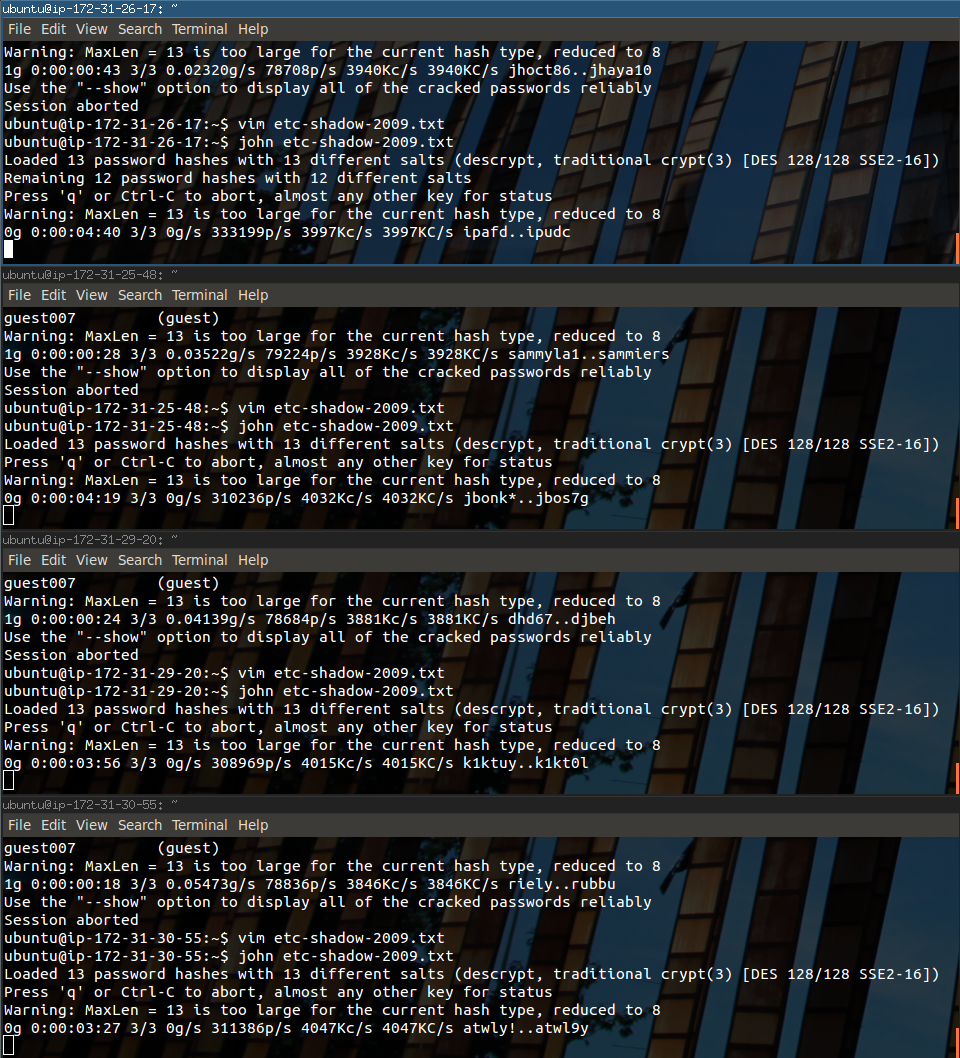
\includegraphics[width=7.5in]{img/t1s1.png}
        }
		\centering
		\caption{Task 1 - Four instances running at once over ssh}
	\end{figure}


\clearpage

\section{Task 2}
I was able to run hashcat on my desktop at home, which natively runs Ubuntu 16.04 (as opposed to my laptop that I `dist-uprade`ed to 16.04), and also includes an NVidia GPU as opposed to my laptop's AMD card.
I attempted to make a docker to see if it would run correctly inside of there, but it suffered from the same drivers issue that I struggled with before, and it didn't seem worth it to install those in the docker, too.
Anyways, I ran the hashcat program twice. Once with attack mode 0:

\begin{verbatim}
eb61eead90e3b899c6bcbe27ac581660:HELLO
2ac9cb7dc02b3c0083eb70898e549b63:Password1
75b71aa6842e450f12aca00fdf54c51d:P455w0rd
2c9341ca4cf3d87b9e4eb905d6a3ec45:Test1234
958152288f2d2303ae045cffc43a02cd:MYSECRET
eb61eead90e3b899c6bcbe27ac581660:HELLO
2ac9cb7dc02b3c0083eb70898e549b63:Password1
75b71aa6842e450f12aca00fdf54c51d:P455w0rd
2c9341ca4cf3d87b9e4eb905d6a3ec45:Test1234
958152288f2d2303ae045cffc43a02cd:MYSECRET
\end{verbatim}

Attack mode 3 (bruteforcing) was insanely slow, and I suspect would not have been able to find all of the passwords anyways, at least not today.
\begin{verbatim}
eb61eead90e3b899c6bcbe27ac581660:HELLO
2ac9cb7dc02b3c0083eb70898e549b63:Password1
75b71aa6842e450f12aca00fdf54c51d:P455w0rd
2c9341ca4cf3d87b9e4eb905d6a3ec45:Test1234
958152288f2d2303ae045cffc43a02cd:MYSECRET
\end{verbatim}

I have not yet completed the android APK

\section{Task 3}
I haven't technically started this yet, however I by creating the docker container for the previous section, I was able to trivially transfer my hashcat setup to the new machine.
To test it, I modified my dockerfile slightly from before:


\begin{verbatim}
FROM hihouhou/hashcat

ADD http://cecs.wright.edu/~pmateti/Courses/3900/Lectures/Assignments/hashes-md5.txt /root/
ADD http://downloads.skullsecurity.org/passwords/rockyou.txt.bz2

RUN apt-get install -y bzip2
RUN cd /root/ && bzip2 -d rockyou.txt.bz2
\end{verbatim}

and then the output:
\begin{verbatim}
[s]tatus [p]ause [r]esume [b]ypass [q]uit =>

Input.Mode: Dict (/root/rockyou.txt)
Index.....: 5/5 (segment), 553093 (words), 5720127 (bytes)
Recovered.: 5/8 hashes, 0/1 salts
Speed/sec.: 4.38M plains, 4.38M words
Progress..: 553093/553093 (100.00%)
Running...: 00:00:00:01
Estimated.: --:--:--:--


Started: Fri Apr  7 04:09:48 2017
Stopped: Fri Apr  7 04:09:53 2017
ubuntu@ip-172-31-26-17:~$
\end{verbatim}

The hashes cracked:
\begin{verbatim}
2ac9cb7dc02b3c0083eb70898e549b63:Password1
eb61eead90e3b899c6bcbe27ac581660:HELLO
75b71aa6842e450f12aca00fdf54c51d:P455w0rd
2c9341ca4cf3d87b9e4eb905d6a3ec45:Test1234
958152288f2d2303ae045cffc43a02cd:MYSECRET
\end{verbatim}


\end{document}
